\documentclass[aspectratio=169,11pt]{beamer}

% ---------- theme & packages ----------
\usetheme{default}
\usecolortheme{seahorse}
\setbeamertemplate{navigation symbols}{}
\setbeamertemplate{footline}[frame number]
\setbeamerfont{frametitle}{size=\Large,series=\bfseries}
\setbeamerfont{title}{size=\huge,series=\bfseries}

\usepackage{listings}
\usepackage{xcolor}
\usepackage{tikz}
\usetikzlibrary{positioning,arrows.meta,shapes.geometric}
\usepackage{fontspec}\ifx\fontspec\undefined\else\setmonofont{Menlo}\fi

\definecolor{codebg}{HTML}{F4F4F6}
\definecolor{kw}{HTML}{2A6F97}
\definecolor{str}{HTML}{2F855A}
\definecolor{com}{HTML}{888888}

\lstdefinelanguage{shell}{morekeywords={curl,GET,POST,export,cd,pip,python3,uvicorn,npm,docker},morecomment=[l]{\#}}
\lstset{
  basicstyle=\ttfamily\small,
  backgroundcolor=\color{codebg},
  keywordstyle=\color{kw}\bfseries,
  commentstyle=\color{com}\itshape,
  stringstyle=\color{str},
  showstringspaces=false,
  breaklines=true, breakatwhitespace=true,
  frame=none, framesep=4pt,
  xleftmargin=4pt, xrightmargin=4pt,
  aboveskip=4pt, belowskip=4pt,
}

\newcommand{\hl}[1]{\textcolor{kw}{\textbf{#1}}}

% ---------- meta ----------
\title{fire\_demo3\_api}
\subtitle{Backend API \& how to build a frontend on it}
\date{}
\author{}

\begin{document}

% --------------------------------------------------------------------
\begin{frame}
  \titlepage
  \begin{center}\small Repo branch: \texttt{backend-v2}\\
  \texttt{https://github.com/jptalusan/fire\_demo3\_api/tree/backend-v2}\end{center}
\end{frame}

% --------------------------------------------------------------------
\begin{frame}{What it is}
  \begin{itemize}\setlength\itemsep{8pt}
    \item FastAPI backend that drives the C++ fire/EMS simulator.
    \item Login with username + password; server returns a session cookie.
    \item Long-running simulations go on a queue; a worker process runs them.
    \item Frontend reads and writes JSON over HTTP.
  \end{itemize}
\end{frame}

% --------------------------------------------------------------------
\begin{frame}{How the pieces fit together}
\vspace{4pt}
\centering
\resizebox{0.92\linewidth}{!}{%
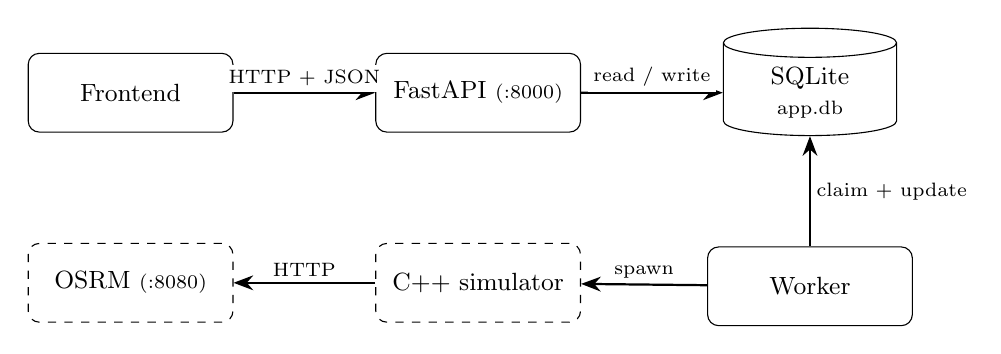
\begin{tikzpicture}[
  node distance=14mm and 18mm,
  proc/.style={draw,rounded corners,minimum height=10mm,minimum width=26mm,align=center,font=\small},
  db/.style={draw,cylinder,shape border rotate=90,aspect=0.3,minimum height=12mm,minimum width=22mm,align=center,font=\small},
  ext/.style={draw,dashed,rounded corners,minimum height=10mm,minimum width=26mm,align=center,font=\small},
  arr/.style={-{Stealth[length=2.5mm]},thick},
  lbl/.style={font=\scriptsize,fill=white,inner sep=2pt},
]
% Row 1, left to right
\node[proc]               (fe)  {Frontend};
\node[proc, right=of fe]  (api) {FastAPI \scriptsize(:8000)};
\node[db,   right=of api] (db)  {SQLite \\ \scriptsize app.db};

% Row 2, RIGHT TO LEFT, columns mirror Row 1 (worker under db, sim under api, osrm under fe)
\node[proc, below=of db]  (w)    {Worker};
\node[ext,  below=of api] (sim)  {C++ simulator};
\node[ext,  below=of fe]  (osrm) {OSRM \scriptsize(:8080)};

\draw[arr] (fe)  -- node[lbl,above]{HTTP + JSON}    (api);
\draw[arr] (api) -- node[lbl,above]{read / write}   (db);
\draw[arr] (w)   -- node[lbl,right]{claim + update} (db);
\draw[arr] (w)   -- node[lbl,above]{spawn}          (sim);
\draw[arr] (sim) -- node[lbl,above]{HTTP}           (osrm);
\end{tikzpicture}}

\vspace{8pt}
\small A frontend only talks to FastAPI. Everything below the API is internal.
\end{frame}

% --------------------------------------------------------------------
\begin{frame}{The two things a frontend must do}
  \begin{enumerate}\setlength\itemsep{12pt}
    \item \hl{Log in once} \;--\; get a session cookie.
    \item \hl{Submit jobs, then poll} \;--\; never block on a long request.
  \end{enumerate}
  \vspace{6pt}
  \small Everything else is shape details (payload \& result).
\end{frame}

% --------------------------------------------------------------------
\begin{frame}{Auth model}
  \begin{itemize}\setlength\itemsep{6pt}
    \item Register \(\rightarrow\) Log in \(\rightarrow\) cookie \texttt{auth\_token} (HttpOnly, 6\,h).
    \item Browser auto-sends it. SPAs use \texttt{credentials: 'include'}.
    \item Non-browser clients: \texttt{Authorization: Bearer <access\_token>}.
    \item Any 401 \(\rightarrow\) prompt re-login.
  \end{itemize}
\end{frame}

% --------------------------------------------------------------------
\begin{frame}[fragile]{Auth — endpoints}
\begin{lstlisting}[language=shell]
POST /auth/register   {username, password}      -> {id, username}
POST /auth/login      {username, password}      -> {access_token, ...} + cookie
GET  /auth/me                                   -> {id, username}
POST /auth/logout                                -> clears cookie
\end{lstlisting}
\vspace{4pt}
\small Rules: username $\geq$3, password $\geq$6. 409 if taken. 401 if wrong.
\end{frame}

% --------------------------------------------------------------------
\begin{frame}{Job lifecycle}
\vspace{4pt}
\centering
\resizebox{0.85\linewidth}{!}{%
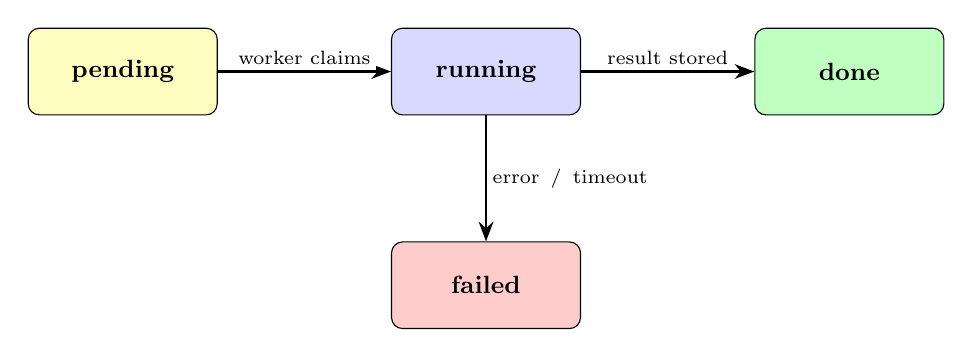
\begin{tikzpicture}[
  node distance=22mm,
  st/.style={draw,rounded corners,minimum height=11mm,minimum width=24mm,font=\small\bfseries,align=center},
  arr/.style={-{Stealth[length=2.5mm]},thick},
  lbl/.style={font=\scriptsize,fill=white,inner sep=2pt},
]
\node[st, fill=yellow!25]                  (p) {pending};
\node[st, fill=blue!15,    right=of p]     (r) {running};
\node[st, fill=green!25,   right=of r]     (d) {done};
\node[st, fill=red!20,     below=16mm of r](f) {failed};

\draw[arr] (p) -- node[lbl,above]{worker claims}      (r);
\draw[arr] (r) -- node[lbl,above]{result stored}      (d);
\draw[arr] (r) -- node[lbl,right]{error \,/\, timeout} (f);
\end{tikzpicture}}

\vspace{12pt}
\begin{itemize}\setlength\itemsep{4pt}
  \item One job runs at a time. Others wait with a \texttt{queue\_position}.
  \item Per-job timeout: 1 hour. Stuck jobs are cleared automatically.
  \item Jobs are saved in the database — a page refresh loses nothing.
\end{itemize}
\end{frame}

% --------------------------------------------------------------------
\begin{frame}[fragile]{Endpoints (16 total)}
\begin{lstlisting}[language=shell,basicstyle=\ttfamily\scriptsize]
# auth
POST /auth/register | POST /auth/login | GET /auth/me | POST /auth/logout

# jobs (the core)
POST /api/jobs                      submit a simulation
GET  /api/jobs                      your job history
GET  /api/jobs/{id}                 one job (with result)
GET  /api/jobs/{id}/progress        live incidents processed
GET  /api/jobs/queue/status         queue snapshot

# inputs / lookups
POST /api/incidents/get-incidents      historical (CSV)
POST /api/incidents/generate-incidents synthetic  (CSV)
POST /api/incidents/process-incidents  stats for a CSV
GET  /api/stations/get-stations        list station CSVs
GET  /api/stations/get-shapes          list geojson overlays

# system
GET /health   GET /version
\end{lstlisting}
\end{frame}

% --------------------------------------------------------------------
\begin{frame}[fragile]{Submit a job — run-simulation}
\begin{lstlisting}[basicstyle=\ttfamily\scriptsize]
POST /api/jobs
{
  "kind": "run-simulation",
  "payload": {
    "models":        { "incident": "historical_incidents",
                       "travelTime": "OSRM",
                       "serviceTime": "ml_based" },
    "date_range":    { "start_date": "2024-06-01",
                       "end_date":   "2024-06-03" },
    "incident_type":   "ems_fire",        // or "fire"
    "dispatch_policy": "nearest",         // or "firebeats"
    "station_data":    "default_stations",// or "custom_stations"
    "disable_ems":     false
  },
  "priority": 0
}
\end{lstlisting}
\vspace{2pt}\small Returns \texttt{\{id, status:"pending", queue\_position, ...\}} instantly.
\end{frame}

% --------------------------------------------------------------------
\begin{frame}[fragile]{Submit a job — run-comparison}
\begin{lstlisting}[basicstyle=\ttfamily\scriptsize]
POST /api/jobs
{
  "kind": "run-comparison",
  "payload": {
    "baseline":  { /* SimConfig — usually default_stations */ },
    "newConfig": { /* SimConfig — your change to evaluate */ }
  }
}
\end{lstlisting}
\vspace{8pt}
\small Both legs run in parallel. Result has \texttt{baseline}, \texttt{newConfig}, and a precomputed \texttt{comparison.overall\_metrics} with $\Delta$ + \texttt{improved} booleans.
\end{frame}

% --------------------------------------------------------------------
\begin{frame}{Custom stations}
  \begin{itemize}\setlength\itemsep{6pt}
    \item Set \texttt{station\_data: "custom\_stations"}.
    \item Provide \texttt{stations: [...]} — each \texttt{\{id, name, lat, lon, apparatus\}}.
    \item Apparatus types: \texttt{Engine, Truck, Rescue, Hazard, Squad, FAST, Medic, Brush, Boat, UTV, REACH, Chief}.
    \item \textbf{Rule}: fire incidents need an Engine; EMS need a Medic. Otherwise the sim won't terminate (will time out and fail).
  \end{itemize}
\end{frame}

% --------------------------------------------------------------------
\begin{frame}[fragile]{Polling: status + live progress}
\begin{lstlisting}[language=shell]
GET /api/jobs/42
  -> { id, status, payload, result, error,
       duration_seconds, queue_position, ... }

GET /api/jobs/42/progress
  -> { status, processed, total, percent,
       legs: { simulation: {processed, total} } }
\end{lstlisting}
\vspace{4pt}
\begin{itemize}\setlength\itemsep{4pt}
  \item Poll every \(\sim\)3\,s while active; 15\,s when idle.
  \item \texttt{percent} reaches 100\% before resolution finishes. Trust \texttt{status}, not the bar.
\end{itemize}
\end{frame}

% --------------------------------------------------------------------
\begin{frame}[fragile]{Result shape — run-simulation}
\begin{lstlisting}[basicstyle=\ttfamily\scriptsize]
{
  "status": "success",
  "total_incidents": 810,
  "average_response_time": 264.06,
  "coverage_percent": 72.84,
  "P90_continuous": 446.2,
  "duration_seconds": 38.16,

  "station_report": [ { "Station 01": { travel_time_mean,
                          incident_count, travel_times[],
                          incident_locations[] } }, ... ],

  "vehicle_report": [ /* per-apparatus metrics */ ],
  "average_response_time_per_incident_type": [ ... ]
}
\end{lstlisting}
\end{frame}

% --------------------------------------------------------------------
\begin{frame}[fragile]{Result shape — comparison summary}
\begin{lstlisting}[basicstyle=\ttfamily\scriptsize]
"comparison": {
  "overall_metrics": {
    "average_response_time": { baseline, new, difference,
                               percent_change, improved },
    "coverage_percent":      { ... },
    "p90_response_time":     { ... }
  },
  "station_comparison":      [ ... per-station deltas ... ],
  "incident_type_comparison":[ ... ],
  "improvements": { response_time_improved,
                    stations_with_better_response, ... },
  "summary": { overall_assessment: "improved|degraded|mixed",
               key_findings: [...] }
}
\end{lstlisting}
\end{frame}

% --------------------------------------------------------------------
\begin{frame}[fragile]{cURL — end to end}
\begin{lstlisting}[language=shell]
B=http://localhost:8000

curl -X POST $B/auth/register -H 'Content-Type: application/json' \
  -d '{"username":"demo","password":"demo-pw1"}'

curl -c jar -X POST $B/auth/login -H 'Content-Type: application/json' \
  -d '{"username":"demo","password":"demo-pw1"}'

JID=$(curl -b jar -X POST $B/api/jobs -H 'Content-Type: application/json' \
  -d @sim.json | jq -r .id)

curl -b jar $B/api/jobs/$JID/progress
curl -b jar $B/api/jobs/$JID    # poll until status=done
\end{lstlisting}
\end{frame}

% --------------------------------------------------------------------
\begin{frame}{Errors to design for}
\small
\begin{tabular}{lll}
\textbf{Code} & \textbf{When} & \textbf{UI} \\\hline
401 & missing / expired session & redirect to login \\
404 & job not yours / not found & 404 view \\
409 & username taken & inline field error \\
422 & request validation & highlight bad field \\
\hline
job \texttt{failed} & runaway / bad config / timeout & show \texttt{error} text \\
\end{tabular}

\vspace{10pt}
\small A failed job is HTTP 200 with \texttt{status:"failed"} and a human \texttt{error}.
\end{frame}

% --------------------------------------------------------------------
\begin{frame}{Run the backend — prereqs}
  \begin{itemize}\setlength\itemsep{6pt}
    \item Python 3.10+.
    \item C++ simulator binary at \texttt{data/fire\_simulator} (executable).
    \item Data assets in \texttt{data/} (incidents, stations, ONNX, geojson).
    \item OSRM reachable (bundled compose runs it on host 8080).
    \item Node 18+ if you'll run the example UI.
  \end{itemize}
\end{frame}

% --------------------------------------------------------------------
\begin{frame}[fragile]{Run it — local}
\begin{lstlisting}[language=shell,basicstyle=\ttfamily\scriptsize]
git clone -b backend-v2 https://github.com/jptalusan/fire_demo3_api.git
cd fire_demo3_api

cp .env.example .env                # edit SECRET_KEY for non-dev
python3 -m venv .venv && source .venv/bin/activate
pip install -e ".[dev]"

set -a && source .env && set +a     # load BACKEND_PORT etc. into shell

# terminal 1
uvicorn backend.main:app --host 0.0.0.0 --port $BACKEND_PORT

# terminal 2
python -m worker.main
\end{lstlisting}
\vspace{2pt}\small Port from \texttt{.env}; change \texttt{BACKEND\_PORT} to use a different one. \texttt{storage/}, \texttt{logs/}, \texttt{data/} auto-created on first start.
\end{frame}

% --------------------------------------------------------------------
\begin{frame}[fragile]{Run it — Docker}
\begin{lstlisting}[language=shell]
cp .env.example .env       # set BACKEND_PORT / OSRM_HOST_PORT here
docker compose up --build
\end{lstlisting}

\vspace{8pt}
\small Brings up \texttt{backend} (\texttt{\$BACKEND\_PORT}, default 8000),
\texttt{worker}, and \texttt{osrm} (\texttt{\$OSRM\_HOST\_PORT}, default 8080).
Host directories mounted: \texttt{./data}, \texttt{./storage}, \texttt{./logs}.
Put data files in \texttt{./data} before \texttt{up}.
\end{frame}

% --------------------------------------------------------------------
\begin{frame}[fragile]{Verify it's alive}
\begin{lstlisting}[language=shell]
curl http://localhost:$BACKEND_PORT/health        # {"status":"ok"}
open  http://localhost:$BACKEND_PORT/docs         # interactive Swagger
curl http://localhost:$BACKEND_PORT/api/v1/openapi.json | head
\end{lstlisting}
\vspace{8pt}\small \texttt{/docs} = best place to explore live. \texttt{/api/v1/openapi.json} = feed to client generators (\texttt{openapi-typescript}).
\end{frame}

% --------------------------------------------------------------------
\begin{frame}[fragile]{Frontend dev against this API}
\begin{lstlisting}[language=shell]
# in your own frontend repo
fetch('http://localhost:8000/api/jobs', {
  method: 'POST',
  credentials: 'include',        // cookie auth
  headers: {'Content-Type':'application/json'},
  body: JSON.stringify({ kind, payload })
})
\end{lstlisting}
\vspace{6pt}
\begin{itemize}\setlength\itemsep{4pt}
  \item Same-site cookie: page host \& API host must match (use \texttt{127.0.0.1} on both, or both \texttt{localhost}).
  \item Generate a typed client:\\\texttt{npx openapi-typescript openapi.json -o api.ts}
\end{itemize}
\end{frame}

% --------------------------------------------------------------------
\begin{frame}{Where to look for details}
  \begin{itemize}\setlength\itemsep{8pt}
    \item \texttt{/docs} \;--\; live Swagger UI with request examples.
    \item \texttt{API\_REFERENCE.md} \;--\; every field, enum, default, full result schemas.
    \item \texttt{README.md} \;--\; running the backend, troubleshooting.
    \item \texttt{/api/v1/openapi.json} \;--\; spec for client generation.
  \end{itemize}
\end{frame}

% --------------------------------------------------------------------
\begin{frame}{Common gotchas}
\scriptsize
\begin{tabular}{p{0.42\textwidth} p{0.50\textwidth}}
\textbf{Symptom} & \textbf{Fix} \\\hline
Job stuck \texttt{pending} & worker not running \\
\texttt{No such file or directory} & data file missing in \texttt{data/} \\
\texttt{Connection refused} to OSRM & wrong \texttt{OSRM\_HOST}/\texttt{OSRM\_PORT} \\
\texttt{Orphaned: no live worker} & old worker crashed; resubmit \\
Job times out after 1\,h & config can't resolve (e.g.\ no Engine for fire) \\
\texttt{401} on every call & session expired; log in again \\
\end{tabular}
\end{frame}

% --------------------------------------------------------------------
\begin{frame}{Summary for a frontend developer}
  \vspace{14pt}
  \begin{itemize}\setlength\itemsep{10pt}
    \item Endpoints + shapes: \texttt{/docs} (live) or \texttt{API\_REFERENCE.md} (text).
    \item Authentication: log in once; send the cookie on every request.
    \item Any long task: POST to \texttt{/api/jobs}, then poll \texttt{/api/jobs/\{id\}} until \texttt{status="done"}.
    \item Generate a client from the spec at \texttt{/api/v1/openapi.json}.
  \end{itemize}
  \vspace{18pt}
  \begin{center}\small Questions?\;\;Open \texttt{/docs} and try the endpoint.\end{center}
\end{frame}

\end{document}
